\documentclass{beamer}
\usepackage{array}
\newcolumntype{M}[1]{>{\centering\arraybackslash}m{#1}}
\newcolumntype{N}{@{}m{0pt}@{}}


\usetheme{default}
\usecolortheme{rose}
\usepackage{hyperref}
\newcommand{\ignore}[1]{}
\newcommand{\pr}{\mathbb{P}}
\newcommand{\E}{\mathbb{E}}
\newcommand{\var}{\text{var}}
\newcommand{\sd}{\text{sd}}
\newcommand{\h}{\widehat}
\newcommand{\TS}{\textit{T}}
\newcommand{\ts}{\textit{t}}

\setbeamerfont{alerted text}{series=\itshape}
\addtobeamertemplate{navigation symbols}{}{%
    \usebeamerfont{footline}%
    \usebeamercolor[fg]{footline}%
    \hspace{1em}%
    \insertframenumber/\inserttotalframenumber
}

\title{Hypothesis Test and Comparison}

% A subtitle is optional and this may be deleted
\subtitle{STAT-UB.0001 Statistics for Business Control}

\author{Ningshan Zhang}
% - Give the names in the same order as the appear in the paper.
% - Use the \inst{?} command only if the authors have different
%   affiliation.

\institute[New York University] % (optional, but mostly needed)
{
  IOMS Department\\
  nzhang@stern.nyu.edu
  \let\thefootnote\relax\footnotetext{\tiny{*  Office Hours: Wed \& Fri 10:00 - 11:30 AM, KMC 8-174}}
}
\date{Aug 2, 2018}
\AtBeginSubsection[]
{
  \begin{frame}<beamer>{Outline}
    \tableofcontents[currentsection,currentsubsection]
  \end{frame}
}

% Let's get started
\begin{document}

%-------------------
\begin{frame}
  \titlepage
\end{frame}


%-------------------
\begin{frame}{Review: CI for Population Mean}
Setup: let $\bar X$ and $S$ be the mean and standard deviation of a random sample of $n$ observations.

\vspace{\stretch{0.2}}
When $n$ is large $(n\geq 30)$ or the population is normal, a $1-\alpha$ CI for population mean $\mu$ is 
\[ (\bar X -{t_{\alpha/2,n-1}} \frac{S}{\sqrt{n}} , \bar X +{t_{\alpha/2,n-1}} \frac{S}{\sqrt{n}}) \]
\begin{itemize}
\item When $n$ is large, $t_{\alpha/2,n-1} \approx z_{\alpha/2}$.
\end{itemize}
\end{frame}

%-------------------
\begin{frame}{Review: CI for Population Proportion}
Setup: let $\h p$ be the sample proportion of a random sample of $n$ observations. 

\vspace{\stretch{0.2}}
When $np \geq 15$ and $n(1-p) \geq 15$, a $1-\alpha$ CI for population proportion $p$ is 
\[
\left( \h p - z_{\alpha/2} \sqrt{\frac{\h p(1-\h p)}{n}},\, 
 \h p + z_{\alpha/2} \sqrt{\frac{\h p(1-\h p)}{n}}\right)
\]
\begin{itemize}
\item In practice, check for $n \h p\geq 15$ and $n (1-\h p) \geq 15$ .
\end{itemize}
\end{frame}

%-------------------
\begin{frame}{Hypothesis Testing}
Often, someone makes a claim about the world, such as 
\begin{itemize}
\item The revenue of a company is normally distributed with mean \$1.5 B and standard deviation \$0.1 B.
\item David throws 10 heads in a roll with a fair coin.
\end{itemize}

\vspace{\stretch{0.2}}
We collect some data, and we want to evaluate the plausibility of that claim in the face of data.
\end{frame}


%-------------------
\begin{frame}{Hypothesis Testing}
Hypothesis:
\begin{itemize}
\item  A statement about the numerical value of a population parameter.
\end{itemize}
\vspace{\stretch{0.2}}
Null Hypothesis ($H_0$):
\begin{itemize}
\item The statement is true.
\end{itemize}
\vspace{\stretch{0.2}}
Alternative Hypothesis ($H_A$):
\begin{itemize}
\item The statement is false.
\end{itemize}
\end{frame}

%-------------------
\begin{frame}{Hypothesis Testing}
Procedure of a hypothesis testing:
\vspace{\stretch{0.2}}
\begin{enumerate}
\item Specify the null ($H_0$) and alternative ($H_a$) hypothesis.
\item Collect a sample, find evidence against $H_0$ in the sample.
\item Make a conclusion:
\begin{itemize}
\item reject $H_0$ if the evidence is strong.
\item otherwise do not reject $H_0$.
\end{itemize}
\end{enumerate}

\vspace{\stretch{0.2}}
Hypothesis tests work like criminal courts: the defendant is presumed innocent, until proven guilty beyond a reasonable doubt.
\end{frame}


%---------
\begin{frame}{Hypothesis Testing for Population Mean}
\begin{itemize}
\item Setup: Population has unknown mean $\mu$. Let $\bar X$ and $S$ be the mean and standard deviation of a random sample of $n$ observations. 
\item Goal: test whether or not $\mu=\mu_0$ for some given value of $\mu_0$.
\end{itemize}

\vspace{\stretch{0.2}}
\textbf{Step 1: Specify the null ($H_0$) and alternative ($H_a$) hypothesis.}
\end{frame}

%---------
\begin{frame}{Test Statistic}
Step 1: $H_0: \mu = \mu_0, \quad H_A: \mu \ne \mu_0$.

\vspace{\stretch{0.05}}
\textbf{Step 2: Collect a sample, find evidence against $H_0$ in the sample.}

\vspace{\stretch{0.2}}
Given a random sample, define the test statistic 
\[
\TS = \frac{\bar X - \mu_0 }{S/\sqrt{n}}.
\]

\begin{itemize}
\item \TS\ is a random variable. (Why?) 
\item If null hypothesis is true, i.e.\ $\mu=\mu_0$, then
\TS\ is t-distributed with df $=n-1$, when $n\geq 30$ or population is normal.
\end{itemize}
\end{frame}

%---------
\begin{frame}{Test Statistic}
\textbf{Step 2: Collect a sample, find evidence against $H_0$ in the sample.}

\vspace{\stretch{0.2}}
Given a random sample, define the test statistic 
\[
\TS = \frac{\bar X - \mu_0 }{S/\sqrt{n}}.
\]

The observed test statistic, \ts\, is the evidence:
\begin{itemize}
\item If $H_0$ is true, it is not very likely to observe extreme values of \ts, such as $\ts\geq 2$ or $\ts \leq -2$.
\item Larger value of $|\ts|$ means stronger evidence against $H_0$.
\end{itemize}
\let\thefootnote\relax\footnotetext{\tiny{* \TS\ is a random variable, \ts\ is its observed value.}}
\end{frame}

%---------
\begin{frame}{p-value}
\textbf{Step 2: Collect a sample, find evidence against $H_0$ in the sample.}
\\\vspace{\stretch{0.2}}
Evidence (test stat.): $\TS = \frac{\bar X - \mu_0 }{S/\sqrt{n}} \sim t_{n-1}$,  \ts\ is the observed value.
\\ \vspace{\stretch{0.3}}
 The p-value tells us how strong is the evidence against $H_0$:
\begin{itemize}
\item If $H_0$ is true, p-value is the probability of getting a test statistic as least as extreme as the one we observed:
\[
\text{p-value}=\pr(|\TS| \geq |\ts|)\text{ under $H_0$}.
\]
\item When the p-value is small, the evidence is strong, and vice versa.
\end{itemize}
\end{frame}

%-------------------
\begin{frame}{Conclusion}
Step 1: Specify the null ($H_0$) and alternative ($H_a$) hypothesis.
Step 2: Collect a sample, find evidence against $H_0$ in the sample.
\textbf{Step 3: Make a conclusion}

\vspace{\stretch{0.2}}
For significance level $\alpha$ (often use $\alpha=0.05$), 
\begin{itemize}
\item reject $H_0$ if the p-value $\leq\alpha$.
\item do not rejct $H_0$ if p-value $> \alpha$.
\end{itemize}
\end{frame}

%-------------------
\begin{frame}{Interpretation of Significance Level $\alpha$}
When $H_0$ is rejected, we say that the result is statistically significant at level $\alpha$. A common choice is $\alpha=0.05$.
\vspace{\stretch{0.2}}
\begin{itemize}
\item Caution: $\alpha$ is not the probability that $H_0$ is true (there is nothing random about $H_0$!)
\item It is possible that $H_0$ is true but we reject it.
\item Rather, $\alpha$ is the probability, or proportion of the time, that a test of this kind would reject $H_0$ when $H_0$ is true.
\end{itemize}
\end{frame}

%-------------------
\begin{frame}{Hypothesis Testing by Rejection Region}
An alternative way of hypothesis testing:
reject $H_0$ if the observed \ts\ falls into a pre-specified \alert{rejection region}.

\begin{itemize}
\item For significance level $\alpha$,
reject $H_0$ when $|\ts| \geq t_{\alpha/2,n-1}$.
\item Thus the rejection region is $(-\infty, -t_{\alpha/2,n-1}] \cup [t_{\alpha/2,n-1},+\infty)$.
\end{itemize}
\vspace{-0.4cm}
\begin{figure}\caption{The rejection region (when $n$ is large, \TS\ is Z-distributed).}
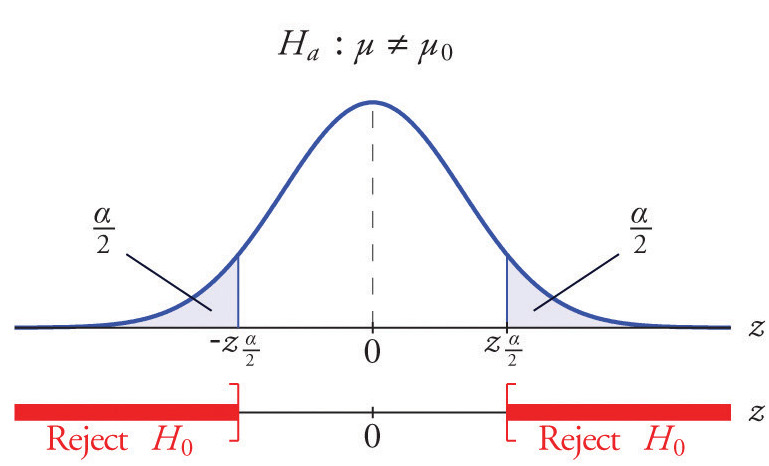
\includegraphics[width=0.5\textwidth]{figures/hypo_test_z.jpg}
\end{figure}
\end{frame}

%-------------------
\begin{frame}{Confidence Intervals and Hypothesis Testing}
%Both rely on the following quantity:
%\begin{equation}\label{eq:T}
%T = \frac{\bar X - \mu}{S/\sqrt{n}}.
%\end{equation}
\begin{itemize}
\item Estimation: A $1-\alpha$ CI for $\mu$ is derived from
$$\frac{\bar X - \mu}{S/\sqrt{n}} \in (-t_{\alpha/2,n-1},t_{\alpha/2,n-1}).$$
%$$\bar X \pm t_{\alpha/2,n-1} \frac{S}{\sqrt{n}}.$$
\item Hypothesis test for $H_0: \mu=\mu_0$ and $H_a:\mu\ne\mu_0$: 
\\ Reject $H_0$ at significance level $\alpha$  when 
$$\frac{\bar X - \mu_0}{S/\sqrt{n}} \not \in (-t_{\alpha/2,n-1},t_{\alpha/2,n-1}).$$
\end{itemize}
\end{frame}


%-------------------
\begin{frame}{Confidence Intervals and Hypothesis Testing}
One can show the following two things are equivalent for a given sample:

\begin{itemize}
\item $\mu_0$ is not in the $1-\alpha$ CI for $\mu$.
\item Reject the $H_0 :\mu=\mu_0$ with significance level $\alpha$;
\end{itemize}

 \vspace{\stretch{0.2}}
Example: given a 95\% CI for $\mu$, and consider the hypothesis test $$H_0: \mu=\mu_0,\quad H_a: \mu \ne \mu_0.$$
If $\mu_0$ is not in the CI, reject $H_0$ with significance 0.05; otherwise do not reject $H_0$.
\end{frame}


%-------------------
\begin{frame}{Types of Errors}
 \begin{table}
 \begin{center}
 \begin{tabular}{|M{3cm}|M{3cm}|M{3cm}|N}
 \hline
 &  $$\text{Reject }H_0$$ & $$\text{Do not reject }H_0$$ \\\hline
 $$H_0\text{ is true}$$ & False positive;\, Type I error & \checkmark \\ \hline
 $$H_0\text{ is false}$$ & \checkmark & False negative; Type II error\\ \hline
 \end{tabular}
 \end{center}
 \end{table}
\let\thefootnote\relax\footnotetext{\tiny{* ''positive'' means reject null. }}
\end{frame}

%-------------------
\begin{frame}{Types of Errors}
Type I Error: Rejecting $H_0$ when $H_0$ is true.
\begin{itemize}
\item Probability of Type I error = ``significance level'' = $\alpha$. 
\end{itemize}

 \vspace{\stretch{0.2}}
Type II Error: Not rejecting $H_0$  when $H_0$ is false.
\begin{itemize}
\item Probability of Type II error = $\beta$.
\item Usually not specified, and can be difficult to calculate.
\end{itemize}

 \vspace{\stretch{0.2}}
Type I and type II errors are conflicting:
\begin{align*}
\text{Decreasing }\alpha & \iff \text{Less likely to reject }H_0 
         \iff \text{Increasing }\beta.
\end{align*}
\end{frame}

%-------------------
\begin{frame}{Comparisons}
Many experiments involve a comparison of two distinct groups.

 \vspace{\stretch{0.2}}
Example:
\begin{itemize}
\item Are men superior drivers?
\item Who has faster 4G LTE network: AT\&T or Verizon?
\item Do SAT prep courses improve scores?
\item Is drug A more effective than drug B (i.e.\ A/B testing)?
\end{itemize}
\end{frame}

%-------------------
\begin{frame}{Comparisons: Setup}
\begin{itemize}
\item There are two populations, let $\mu_k, \sigma_k$ indicate the population mean and standard deviation, for population $k=1,2$.
\item There are two independent random samples from each population, let $n_k, \bar X_k, S_k$ indicate the sample size, sample mean, sample deviation, for population $k=1,2$.
\end{itemize}
 \begin{table}
 \begin{center}
 \begin{tabular}{|M{3cm}|M{3cm}|M{3cm}|N}
 \hline
 & Population 1 & Population 2 \\ \hline
Population parameters & $ \mu_1, \sigma_1 $ & $\mu_2, \sigma_2$  \\\hline
Sample statistics & 
$$n_1,  \bar X_1, S_1$$ &
$$n_2,  \bar X_2, S_2$$ \\\hline
 \end{tabular}
 \end{center}
 \end{table}
 \end{frame}

%-------------------
\begin{frame}{Comparisons: Goal}
Given the sample statistics, we would like to 

\vspace{\stretch{0.2}}
\begin{itemize}
\item Estimation: construct a confidence interval for $\mu_1 - \mu_2$.
\item Hypothesis Testing: test 
$$H_0: \mu_1=\mu_2, \quad H_a: \mu_1 \ne \mu_2.$$
It is equivalent to test
$$H_0: \mu_1-\mu_2=0, \quad H_a: \mu_1 - \mu_2\ne 0.$$

\end{itemize}
 \end{frame}
 
%-------------------
\begin{frame}{Review One Sample Case}
When there is only one sample, we rely on the distribution of
\begin{equation}\label{eq:T}
T = \frac{\bar X - \mu}{S/\sqrt{n}}.
\end{equation}
\begin{itemize}
\item Estimation: A $1-\alpha$ CI for $\mu$ is derived from
$$T \in (-t_{\alpha/2,n-1},t_{\alpha/2,n-1}).$$
%$$\bar X \pm t_{\alpha/2,n-1} \frac{S}{\sqrt{n}}.$$
\item Hypothesis test  for $H_0: \mu=\mu_0$ and $H_a:\mu\ne\mu_0$,
$$\text{Reject $H_0$ when }T \not \in (-t_{\alpha/2,n-1},t_{\alpha/2,n-1}),$$
with $\mu=\mu_0$ in~\eqref{eq:T}.
\end{itemize}
\end{frame}

%-------------------
\begin{frame}{Review One Sample Case}
The key formula is
\[
T = \frac{\bar X - \mu}{S/\sqrt{n}} = \frac{\bar X - \E (\bar X)}{\sd(\bar X)}.
\]

\vspace{\stretch{0.2}}
Given an estimate $\bar X$ of $\mu$, we need to know:
\begin{itemize}
\item Its mean $\E(\bar X)$ and standard deviation $\sd(\bar X)$;
\item The estimate is approximately t or Z distributed.
\end{itemize}
\end{frame}

%-------------------
\begin{frame}{Comparison}
To study $\mu_1-\mu_2$, we need to find:
\begin{itemize}
\item An esitmate of $\mu_1-\mu_2$. Solution:
$$ \bar X_1 - \bar X_2.$$
\item The mean of the estimate. Solution:
$$\E (\bar X_1 - \bar X_2) = \mu_1-\mu_2.$$
\item The standard deviation of the estimate. Solution:
$$\sd (\bar X_1 - \bar X_2) = ? $$
\end{itemize}
\end{frame}

%-------------------
\begin{frame}{Standard Deviation of $\bar X_1 - \bar X_2$}
\begin{block}{Theorem}
If $X,Y$ are two independent random variables, then $$\var(X\pm Y)=\var(X)+\var(Y).$$
\end{block}
Thus,
\begin{align*}
\var(\bar X_1 - \bar X_2) & = \var(\bar X_1) + \var(\bar X_2) = \frac{\sigma_1^2}{n_1} + \frac{\sigma_2^2}{n_2} \\
\Rightarrow \, \sd(\bar X_1 - \bar X_2) & = \sqrt{\frac{\sigma_1^2}{n_1} + \frac{\sigma_2^2}{n_2} }
\end{align*}
Finally, use $\sqrt{\frac{S_1^2}{n_1} + \frac{S_2^2}{n_2} }$ as an estimate for $\sqrt{\frac{\sigma_1^2}{n_1} + \frac{\sigma_2^2}{n_2} }$.
\end{frame}

%-------------------
\begin{frame}{Comparison}
Assume
\begin{itemize}
\item Two independent random samples;
\item Samples are sufficiently large ($n_1\geq30$ and $n_2\geq30$).
\end{itemize}

\vspace{\stretch{0.2}}
Then 
\[
\frac{(\bar X_1 -\bar X_2) - (\mu_1 - \mu_2) }{\sqrt{\frac{S_1^2}{n_1} + \frac{S_2^2}{n_2} }}
\]
is approximately Z distributed.
\let\thefootnote\relax\footnotetext{\tiny{* For comparisons, we only consider the large sample case.}}
\end{frame}

%-------------------
\begin{frame}{Comparison}
\begin{itemize}
\item Estimaton: the $1-\alpha$ CI for $\mu_1 - \mu_2$ is 
$$
(\bar X_1 -\bar X_2) \pm z_{\alpha/2} \sqrt{\frac{S_1^2}{n_1} + \frac{S_2^2}{n_2} }.
$$
\item Hypothesis test for $H_0: \mu_1 = \mu_2$ and  $H_a: \mu_1 \ne \mu_2$:
$$
\text{Reject $H_0$ when } 
\frac{(\bar X_1 -\bar X_2) }{\sqrt{\frac{S_1^2}{n_1} + \frac{S_2^2}{n_2} }} \not \in (-z_{\alpha/2},z_{\alpha/2})
$$
at significance level $\alpha$.
\end{itemize}
\end{frame}


\ignore{
%-------------------
\begin{frame}{Time Series Plot}
\begin{figure}
    \caption{}
    
\includegraphics[width=1\textwidth]{figures/coindesk-bpi-chart}
\end{figure}
\let\thefootnote\relax\footnotetext{\tiny{* Plot from Coindesk.com}}
\end{frame}

\begin{frame}{}
\begin{itemize}
\item 
\end{itemize}
\end{frame}

\vspace{\stretch{0.5}}

\begin{block}{}
\end{block}


}

\end{document}


